\documentclass[cameraready]{Interspeech}

\title{Image Classification with Convolutional Neural Networks on CINIC-10}

\author[affiliation={1}]{Pawel}{Pozorski}
\author[affiliation={1}]{Pawel}{Florek}

\address{
    $^1$ Warsaw University of Technology, Poland
}

\email{\{pawel.pozorski, pawel.florek\}.stud@pw.edu.pl}

\keywords{image classification, convolutional neural networks, CINIC-10, neural architecture search, few-shot learning}

\begin{document}

\maketitle

\begin{abstract}
This paper presents a comparative study of convolutional neural network pipelines for image classification on CINIC-10. We evaluate lightweight and high-capacity backbones, including MobileNetV3 Small, SqueezeNet, ResNet-18, DenseNet-121, and a differentiable NAS-CNN variant. We also test ConvKAN layers as convolutional replacements in efficient models. The study includes a controlled hyperparameter search, modern augmentation methods, reduced-data training, and few-shot metric learning with Prototypical Networks. Experiments are designed for reproducibility with fixed seeds and unified training scripts. We report benchmark context, evaluation protocol, and implementation details that support transparent comparison across model families and training regimes.
\end{abstract}

\section{Introduction}
Convolutional neural networks (CNNs) \cite{lecun1998gradient} remain a practical foundation for image recognition \cite{liu2022convnet}, but model selection is highly task- and constraint-dependent \cite{bianco2018benchmark, tan2019efficientnet}. In this project, we study how different CNN paradigms perform on CINIC-10 \cite{cinic}, a dataset that preserves CIFAR-like \cite{krizhevsky2009learning} image size while increasing distributional complexity via ImageNet-derived \cite{deng2009imagenet} samples.

Compared with CIFAR-10, CINIC-10 introduces a stronger distribution shift because class semantics are preserved while image statistics are broadened by downsampled ImageNet content \cite{cinic}. This makes the benchmark less prone to narrow in-distribution overfitting and more informative for robustness-oriented evaluation. In practice, models that perform similarly on CIFAR-like data may diverge on CINIC-10 once they are exposed to larger intra-class variation, background diversity, and texture/illumination changes \cite{cinic, recht2019do}.

Our goals are threefold: (i) compare efficient and high-capacity architectures under a common training framework, (ii) evaluate whether ConvKAN-style convolutions improve compact models, and (iii) analyze robustness in low-data conditions using subset training and few-shot learning.

\section{Methodology}
\subsection{Dataset}
CINIC-10 \cite{cinic} contains $270{,}000$ RGB images at $32 \times 32$ resolution and $10$ balanced classes \cite{cinic}. samples from the dataset are illustrated in Figure \ref{fig:sample_img}. Data is organized into train, validation, and test splits of $90{,}000$ samples each. The inclusion of ImageNet-derived examples increases intra-class variation relative to CIFAR-10 and makes generalization analysis more informative \cite{cinic}. For the purpose of these experiments, the dataset was sourced from the \texttt{mengcius/cinic10} repository via the Kaggle API, ensuring a standardized pipeline for data loading and preprocessing.

\begin{figure}
    \centering
    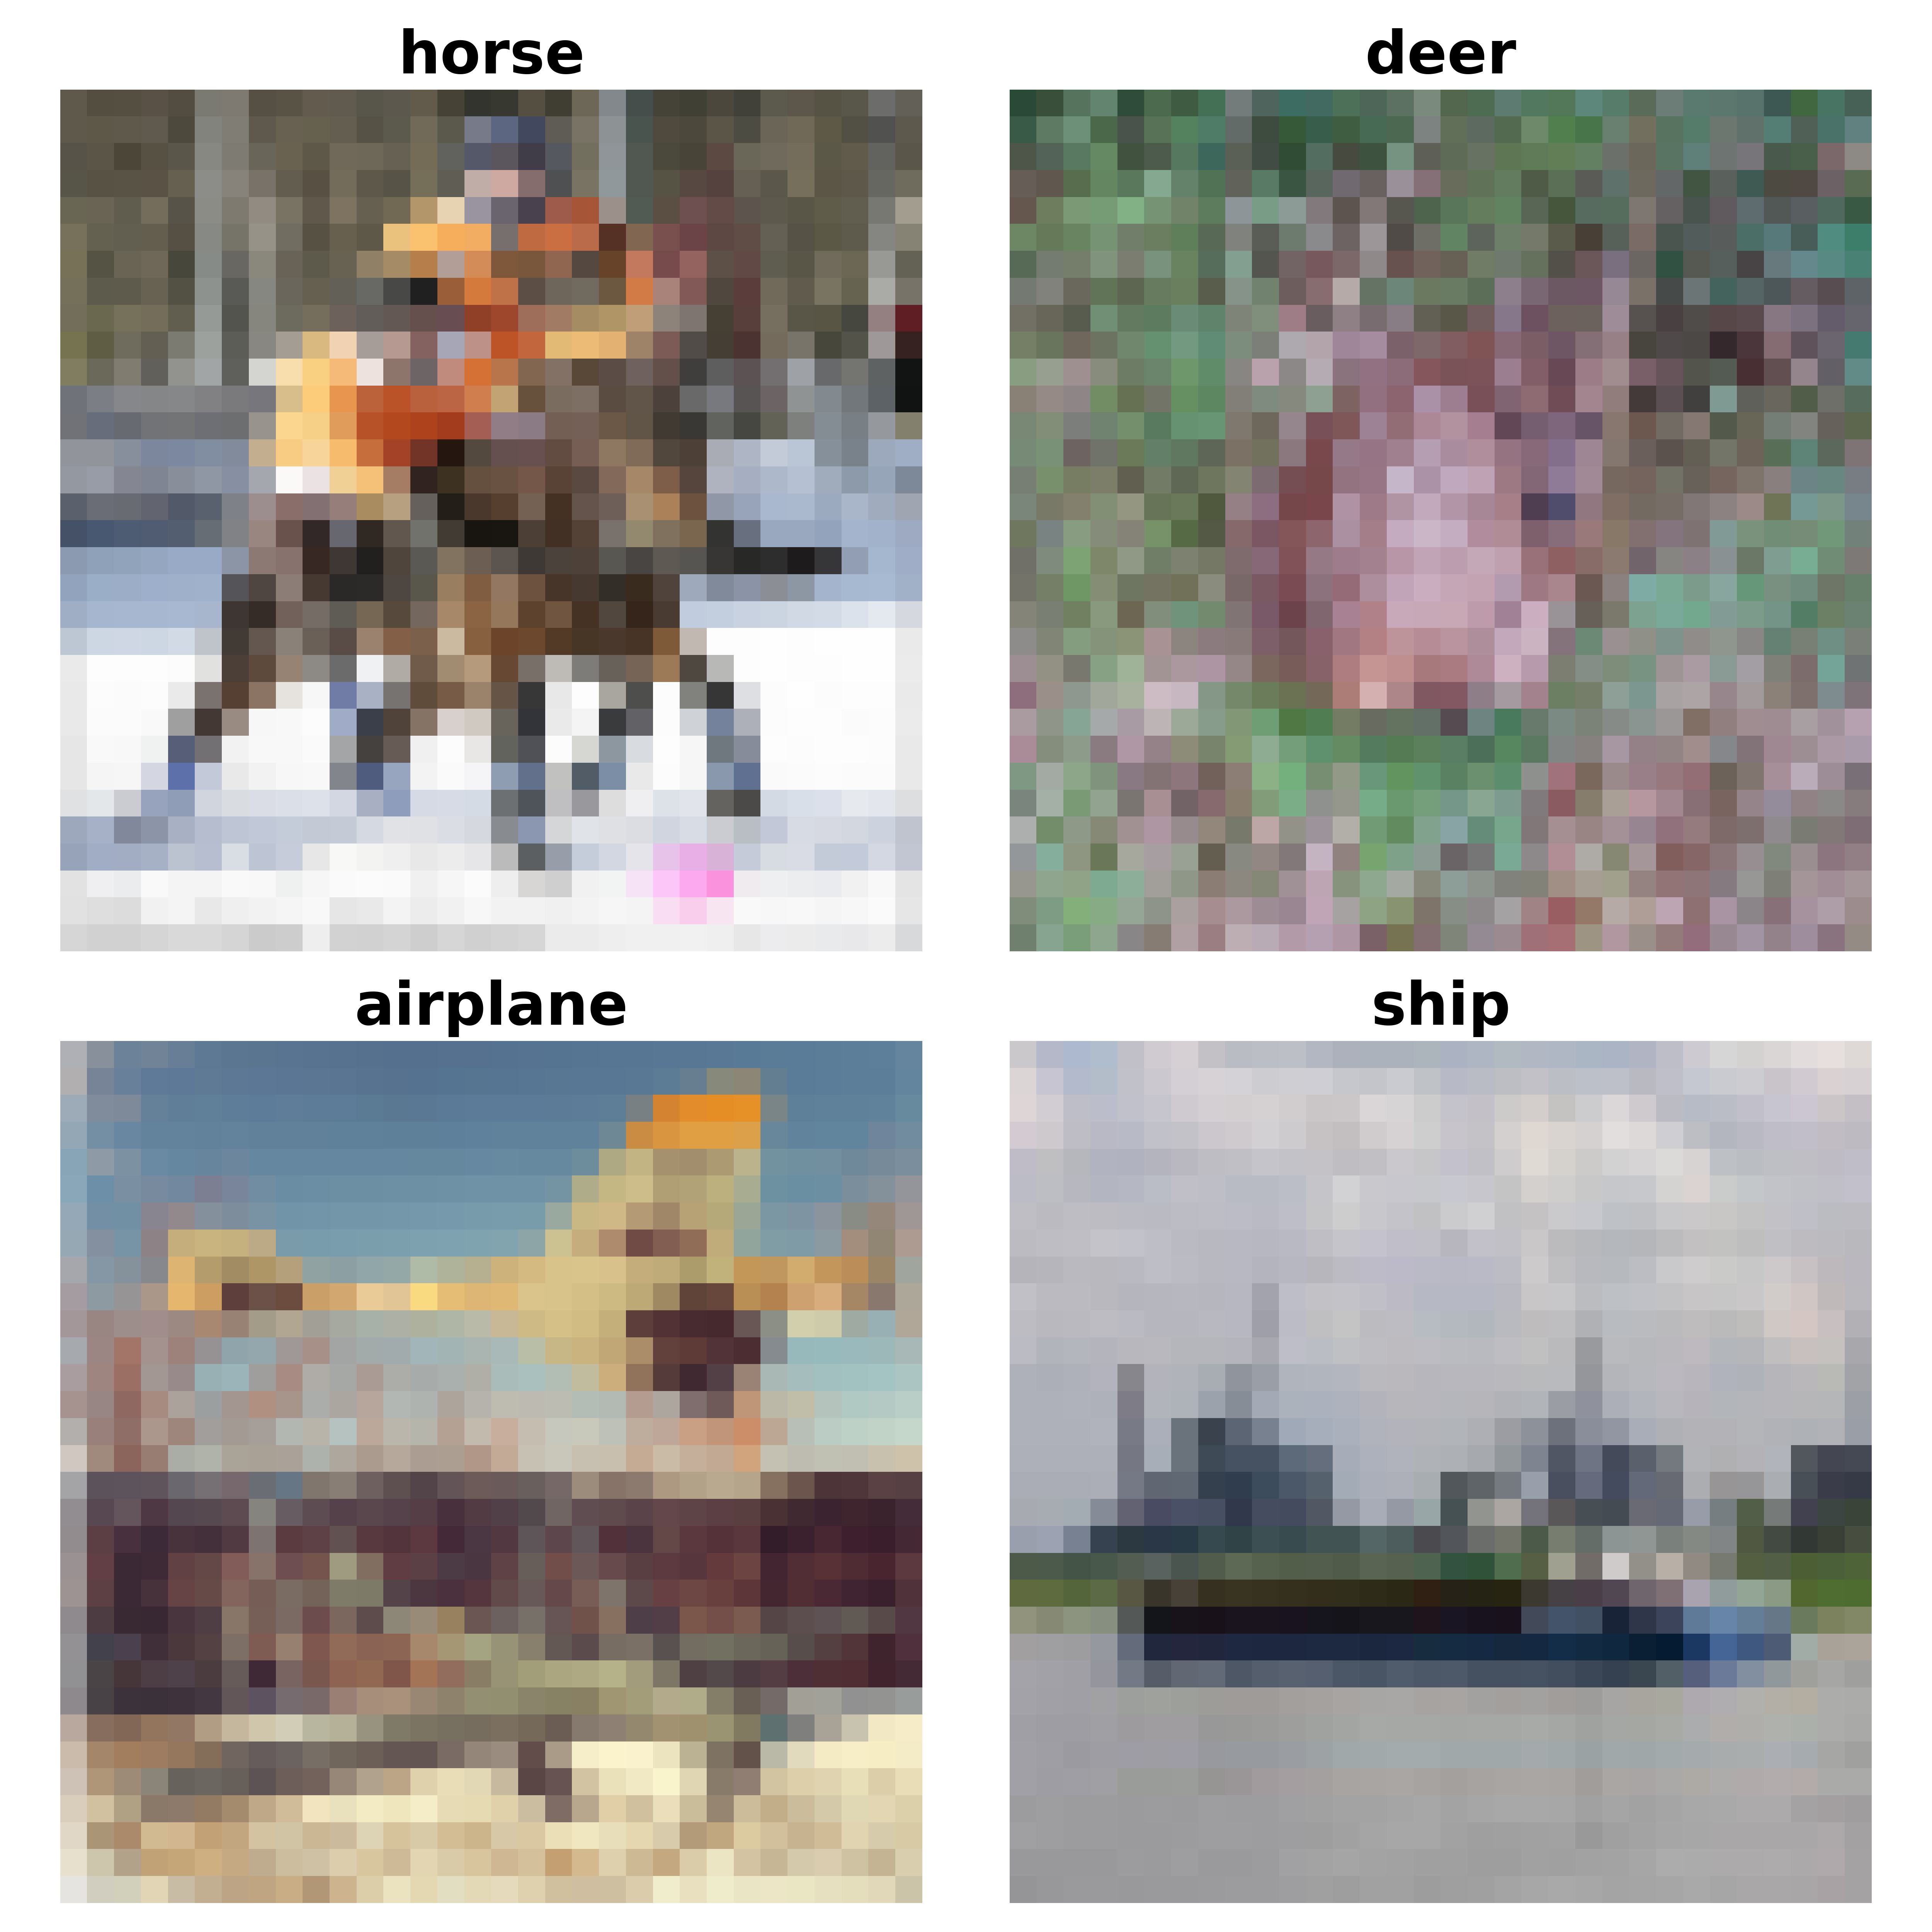
\includegraphics[width=\linewidth]{../src/cinic10/eda/plots/sample_images.png}
    \caption{Example images from CINIC-10 for four classes.}
    \label{fig:sample_img}
\end{figure}



\subsection{Model families}
We evaluate three groups:
\begin{itemize}
    \item \textbf{Search-based architecture}: a differentiable one-shot NAS-CNN supernet with architecture parameters optimized jointly with weights \cite{SalmaniPourAvval2025_nas}.
    \item \textbf{Efficient backbones}: MobileNetV3 Small \cite{Howard_2019_ICCV} and SqueezeNet \cite{SqueezeNet}, including ConvKAN substitutions \cite{10681070_kan}.
    \item \textbf{Transfer baselines}: ResNet-18 \cite{He_2016_CVPR_res} and DenseNet-121 \cite{Huang_2017_CVPR_dense} adapted for the CINIC-10 label space.
\end{itemize}

For ConvKAN variants, we replace eligible spatial convolution layers with \texttt{torchkan}-provided \cite{torchkan} ConvKAN layers while preserving layer shape and stride constraints. Conceptually, this swaps standard linear convolutional kernels for KAN-style parameterization with learnable nonlinear basis behavior on connections, motivated by recent work on Kolmogorov-Arnold Networks \cite{liu2024kan,10681070_kan}. Unlike standard convolutions, which apply fixed scalar weights followed by a static, node-wise activation function (e.g., $y = \text{tanh}(\sum w_i x_i)$), KANs shift the nonlinearity directly to the network edges. In a ConvKAN layer, the scalar elements of a traditional convolutional kernel are replaced by learnable 1D nonlinear functions, typically parameterized as B-splines.  Consequently, each connection applies a dynamic, finely-tuned activation $\phi(x)$ to the input pixels within the receptive field, and the output node simply sums these transformed signals ($y = \sum \phi_i(x_i)$). This theoretical increase in per-parameter expressivity aims to allow lightweight architectures to capture complex spatial patterns more efficiently than standard linear filters.

For NAS, our supernet is constructed as a sequence of searchable edges, formulated via a continuous relaxation of the discrete architecture space \cite{liu2018darts}.  Instead of selecting a single operation, the output of each edge during the search phase is computed as a weighted sum of all candidate operations $o \in \mathcal{O}$, combined using a softmax distribution over learnable architecture parameters $\alpha$:
$$ \bar{o}(x) = \sum_{o \in \mathcal{O}} \frac{\exp(\alpha_o)}{\sum_{o'} \exp(\alpha_{o'})} o(x) $$

Our specific search space $\mathcal{O}$ consists of $5$ candidate operations designed to balance capacity and efficiency: standard convolutions (\texttt{conv3x3}, \texttt{conv5x5}), parameter-efficient \texttt{depthwise3x3}\footnote{A depthwise convolution does not share weights across channels - it learns a distinct spatial filter for each input channel. For example, given an input with $32$ channels, a standard $3\times3$ convolution computing $32$ output channels requires $32 \times 32 \times 3 \times 3 = 9{,}216$ parameters to mix all spatial and channel information simultaneously. A depthwise $3\times3$ layer requires only $32 \times 3 \times 3 = 288$ parameters, as it applies exactly one unique $3\times3$ filter to each input channel independently.}, spatial reduction \texttt{maxpool3x3\_proj}, and identity mapping \texttt{skip\_proj}. The \texttt{\_proj} variants explicitly incorporate a $1 \times 1$ pointwise convolution to ensure tensor dimensions match when spatial strides or channel counts shift across an edge.

The macro-architecture skeleton restricts the search to $6$ sequential edges, following a standard hierarchical feature pyramid defined by these input/output channel ($C_{in} \rightarrow C_{out}$) and stride ($s$) transitions:
\begin{itemize}
    \item $(3\rightarrow32, s=1)$, $(32\rightarrow32, s=1)$, $(32\rightarrow64, s=2)$,
    \item $(64\rightarrow64, s=1)$, $(64\rightarrow128, s=2)$, $(128\rightarrow128, s=1)$.
\end{itemize}
This formulation enables the joint gradient-based optimization of both the network weights and the architecture parameters $\alpha$. Following the search stage, the continuous edge mixtures are discretized by taking the $\arg\max$ of the architecture logits to derive the final feature transformation and downsampling pattern.

\subsection{Training and search setup}
A structured grid search is used for MobileNetV3 Small with the Cartesian product of:
\begin{itemize}
    \item optimizer $\in \{$SGD \cite{bottou2010large}, AdamW \cite{adamw}$\}$,
    \item batch size $\in \{128, 256\}$,
    \item dropout $\in \{0.0, 0.1, 0.5\}$,
    \item weight decay $\in \{0.0, 10^{-4}\}$.
\end{itemize}

These bounds were selected to bracket key training regimes: batch sizes of $128$ and $256$ balance computational efficiency with the implicit regularization of stochastic mini-batch noise \cite{masters2018revisiting}, while the dropout values evaluate whether a lightweight architecture requires no explicit regularization ($0.0$), mild feature decorrelation ($0.1$), or classic aggressive dropout ($0.5$) \cite{srivastava2014dropout}. This yields $24$ configurations per seed in Stage 1 (refer to Section~\ref{sec:execution_plan} for details). This stage is repeated for three fixed seeds $\{0, 42, 3407\}$, resulting in $72$ total runs; thus, seed is treated as an experimental repeatability axis (for stability statistics), not as a tuned hyperparameter. For NAS optimization, temperature annealing and entropy regularization are applied to architecture logits to move from exploratory mixtures to sharper operation selection.

\subsection{Reproducibility and seed control}
The same seed policy is applied consistently across all stages in the execution plan (grid search, augmentation ablation, architecture comparison, NAS two-stage, reduced-data training, and few-shot episodes). One top-level seed initializes Python, NumPy \cite{harris2020array}, and PyTorch \cite{NEURIPS2019_9015} RNG states at process start. Dataloader randomness is controlled with split-specific seeded generators (train/validation/test offsets), so ordering is deterministic within a run but decorrelated across splits. In multi-worker loading, each worker receives a deterministic derived seed and forwards it to Python and NumPy RNGs inside that worker process.

This seed is also propagated to class-stratified subset sampling and few-shot episode construction, so data selection, task generation, augmentation sampling, and batch shuffling are all reproducible for a given run directory (e.g., \texttt{seed\_0}, \texttt{seed\_42}, \texttt{seed\_3407}). Reporting across these seeds provides mean/variance-style stability evidence rather than a single-point estimate.

\subsection{Data augmentation}
The training pipeline includes geometric and photometric transforms and mixing-based regularization:
\begin{itemize}
    \item random rotation, horizontal flip, color jitter;
    \item MixUp \cite{zhang2018mixupempiricalriskminimization}: two samples $(x_i, y_i)$ and $(x_j, y_j)$ are linearly combined as $\tilde{x}=\lambda x_i+(1-\lambda)x_j$ and $\tilde{y}=\lambda y_i+(1-\lambda)y_j$, where the interpolation weight $\lambda \in [0, 1]$ is sampled from a Beta distribution, $\lambda \sim \text{Beta}(\alpha, \alpha)$. This continuous mixing smooths decision boundaries and reduces overconfident predictions. For our experiments, we set $\alpha=0.1$ as it is a pytorch-default;
    \item CutMix \cite{Yun_2019_ICCV_cutmix}: a rectangular patch from one image replaces the corresponding region in another image. The bounding box is determined by a combination ratio $\lambda$ (sampled from a Beta distribution identically to MixUp), with its center uniformly sampled across the spatial dimensions and its width and height scaled proportionally to $\sqrt{1-\lambda}$. Labels are mixed by the exact visible area ratio, encouraging localized evidence use and improving robustness to occlusion. Examples of MixUp and CutMix is shown on the figure \ref{fig:aug_mixing};
    \item AutoAugment (CIFAR-10 policy) \cite{Cubuk_2019_CVPR}: an augmentation schedule originally discovered via reinforcement learning. For each training sample, one sub-policy is uniformly sampled from a pool of $25$ learned policies. Each sub-policy sequentially applies two operations (ranging from geometric transformations like shearing to photometric ones like solarization or color inversion), each with a fixed, optimized probability and magnitude. This automated diversification prevents overfitting more effectively than static, hand-crafted heuristics. Comparison between chosen basic transform methods and AutoAugment is shown on the figure \ref{fig:basic_aug};
\end{itemize}

\begin{figure}
    \centering
    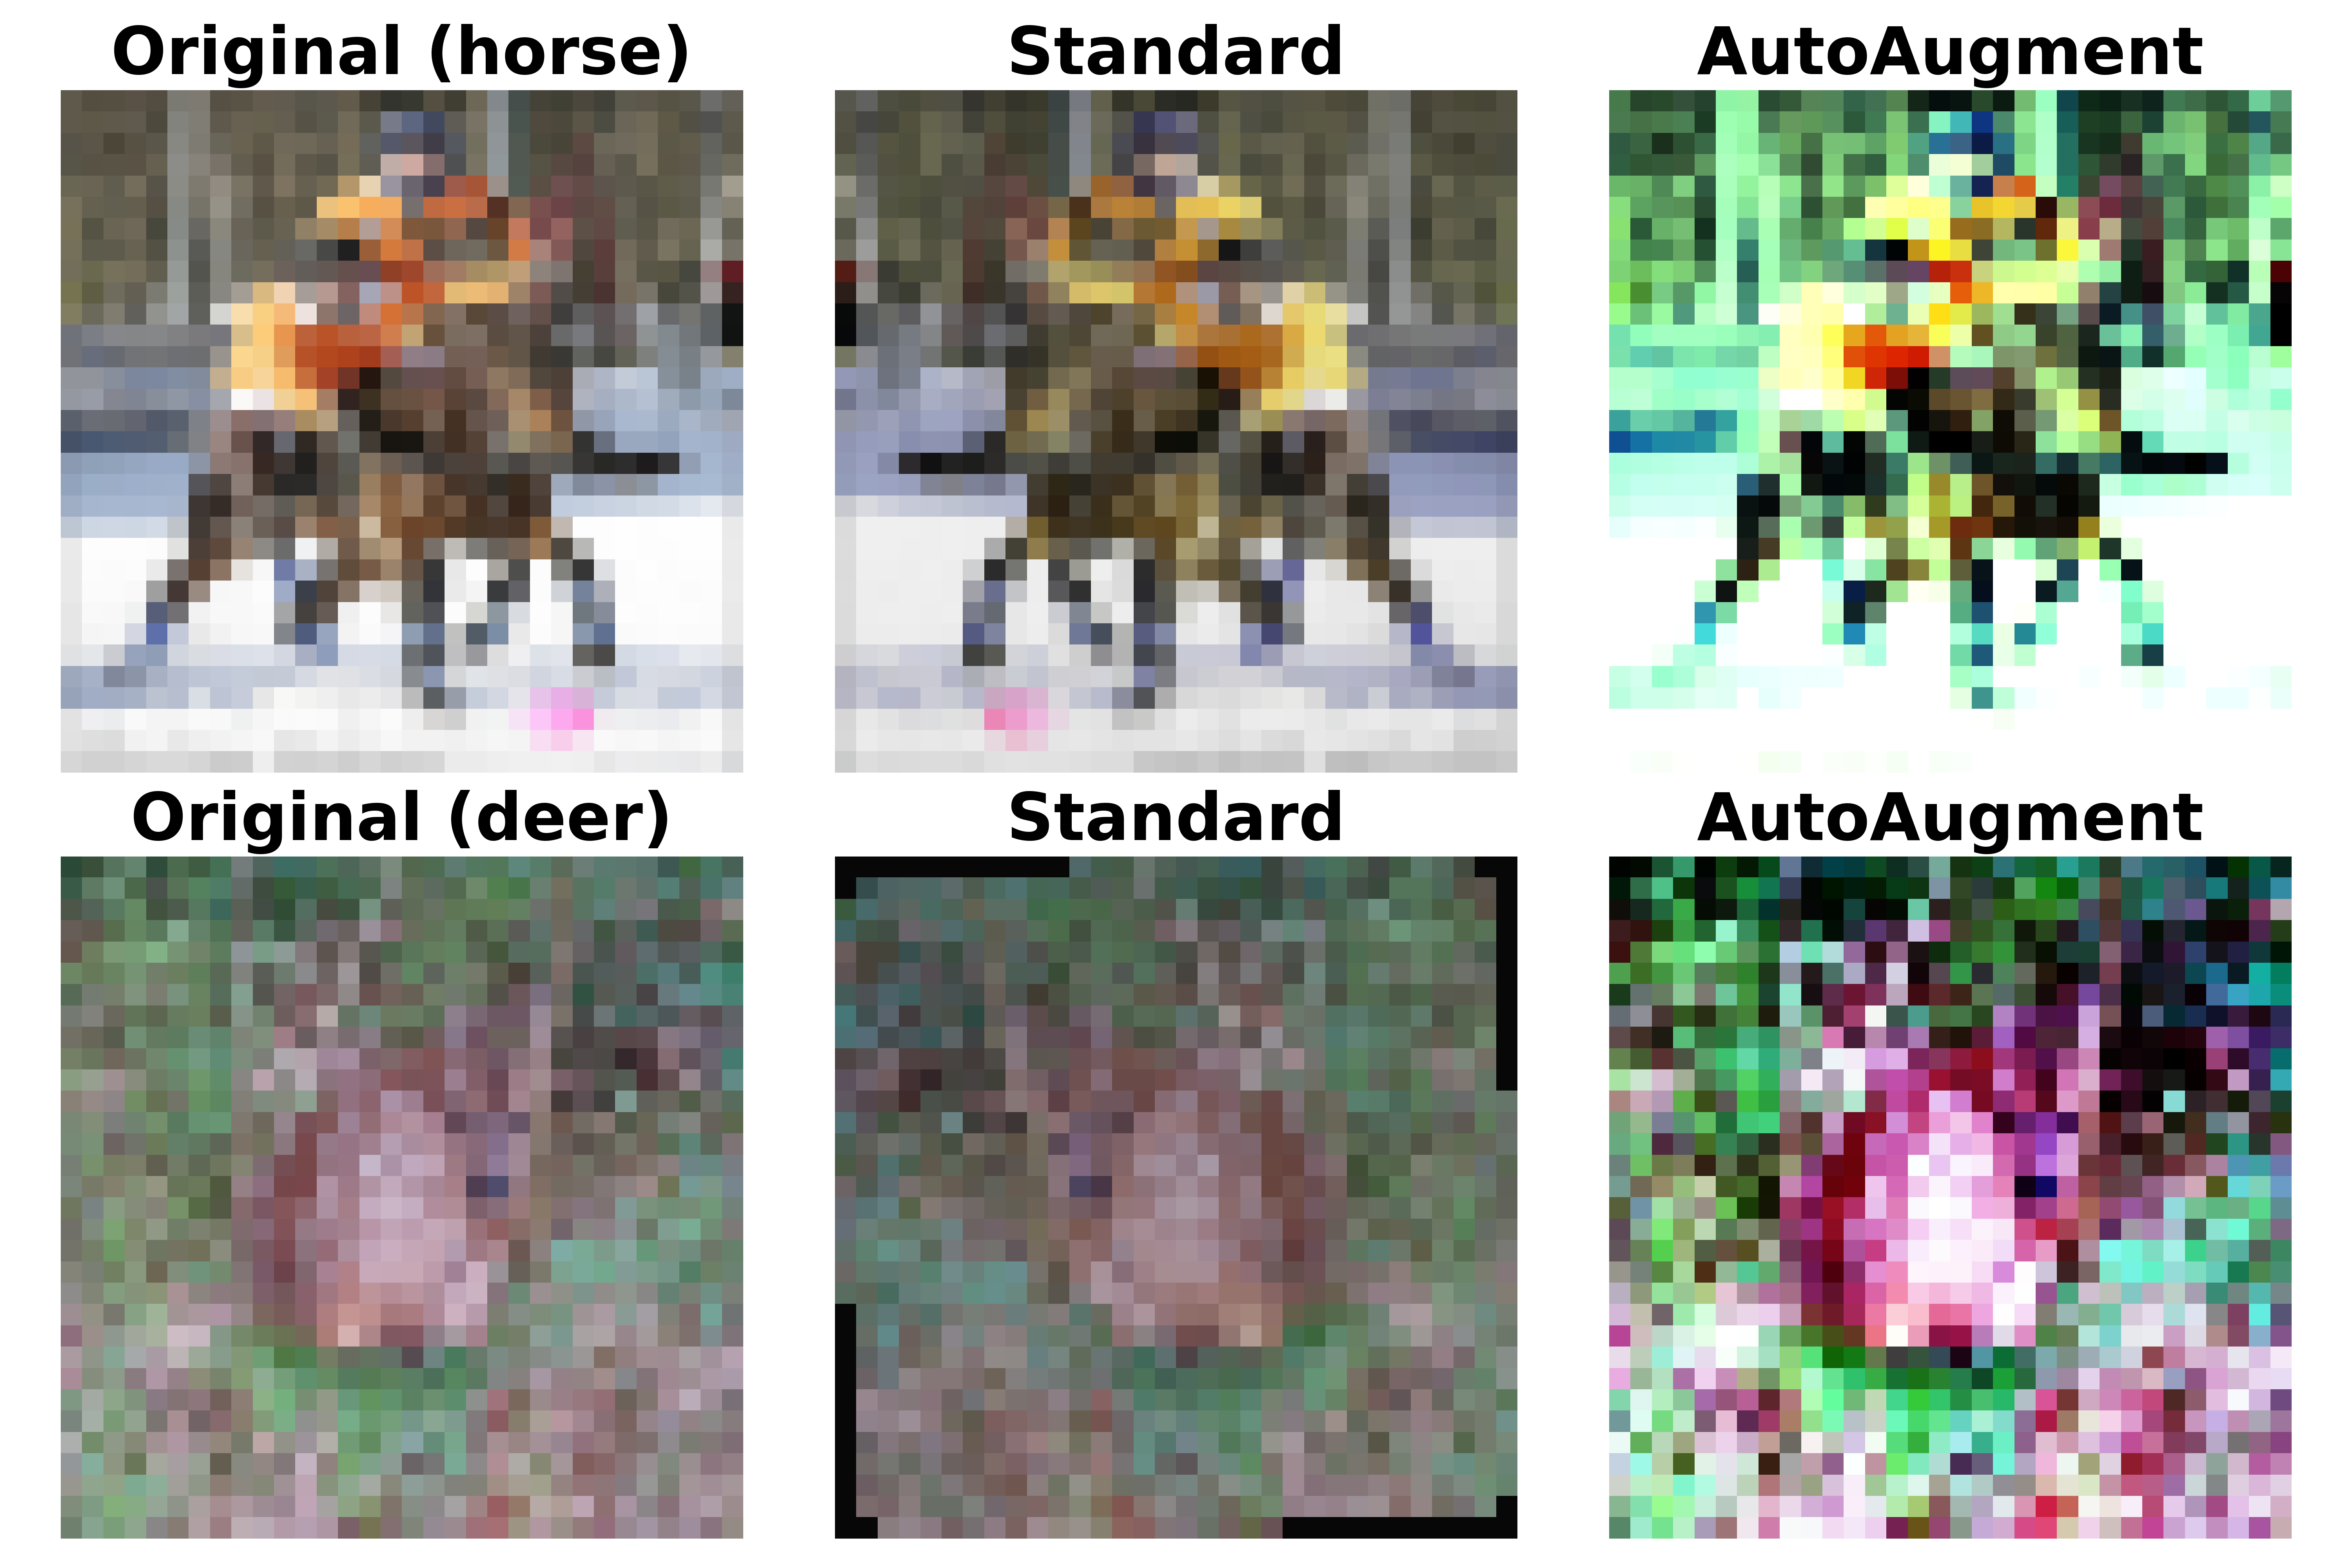
\includegraphics[width=\linewidth]{../src/cinic10/eda/plots/augmentation_sample.png}
    \caption{Showcase of basic augmentation methods and autoaugment.}
    \label{fig:basic_aug}
\end{figure}

\begin{figure}
    \centering
    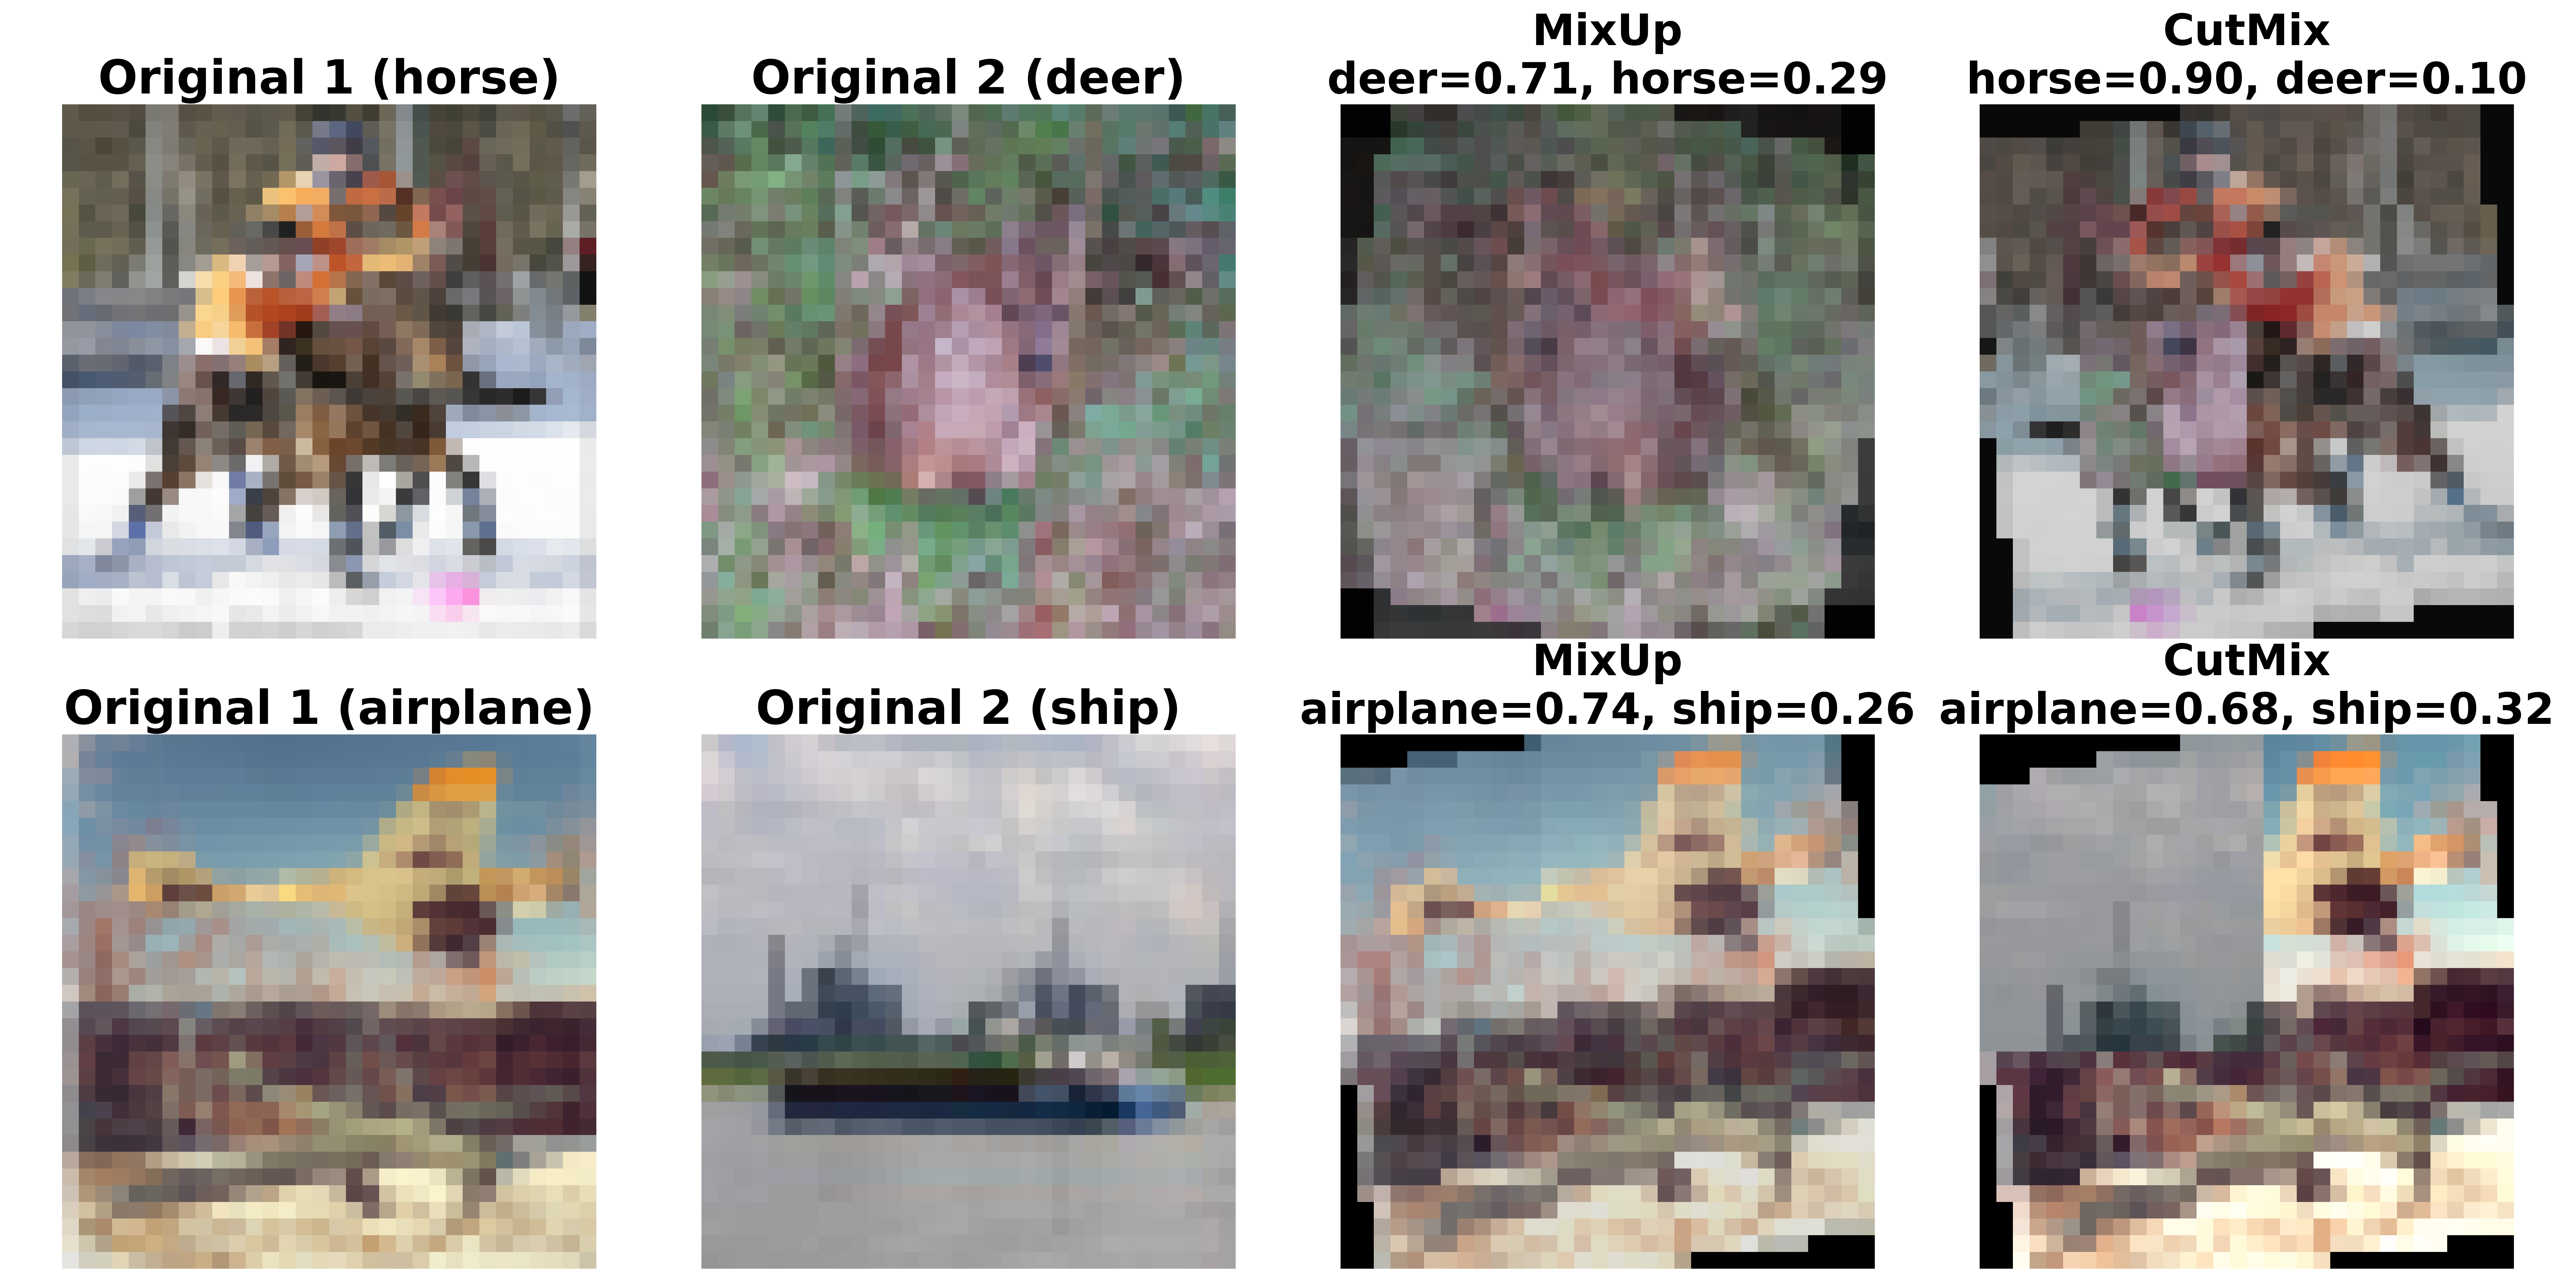
\includegraphics[width=\linewidth]{../src/cinic10/eda/plots/mixing_methods.png}
    \caption{Showcase of mixing methods.}
    \label{fig:aug_mixing}
\end{figure}

\subsection{Low-data evaluation}
Two complementary low-resource protocols are used:
\begin{itemize}
    \item \textbf{Subset training}: supervised training on $5\%$ of data per class, sampled with class-stratified selection. For each class, indices are sampled independently without replacement using the experiment seed, with at least one sample retained per class; this preserves class coverage and prevents label-frequency drift that appears in naive global subsampling.
    \item \textbf{Few-shot learning}: episodic training with Prototypical Networks \cite{NIPS2017_cb8da676}. To optimize the model for transferable class separation rather than closed-set classification, training proceeds through $N$-way, $K$-shot episodes. Each episode is constructed and evaluated through the following steps:
    \begin{enumerate}
        \item \textbf{Task sampling}: A support set $S$ is formed by randomly sampling $N$ classes from the training split and $K$ images per class. A disjoint query set $Q$ is then sampled from those exact same $N$ classes to serve as the episodic test set.
        \item \textbf{Latent embedding and prototype calculation}: The CNN backbone, parameterized by $\theta$, acts as an embedding function $f_\theta$ that maps images into a continuous latent space. For each class $c$, a prototype vector $\mathbf{v}_c$ is computed as the mean of its $K$ embedded support examples:
        $$ \mathbf{v}_c = \frac{1}{K} \sum_{(x_i, y_i) \in S_c} f_\theta(x_i) $$
        \item \textbf{Distance formulation}: Query images $x_q \in Q$ are passed through the same backbone $f_\theta$. The network evaluates the squared Euclidean distance $d$ between the query embedding $f_\theta(x_q)$ and each class prototype $\mathbf{v}_c$.
        \item \textbf{Prediction and optimization}: A softmax function over the negative Euclidean distances yields a probability distribution over the $N$ episodic classes:
        $$ p(y=c|x_q) = \frac{\exp(-d(f_\theta(x_q), \mathbf{v}_c))}{\sum_{c'} \exp(-d(f_\theta(x_q), \mathbf{v}_{c'}))} $$
        The model weights $\theta$ are updated via backpropagation by minimizing the negative log-probability (cross-entropy loss) of the true query labels.
    \end{enumerate}
    By continually optimizing this distance-based metric across varying episodic tasks, the network learns a generalized feature space where intra-class samples cluster tightly, making it highly effective for low-data adaptation on unseen data distributions.
\end{itemize}

\section{Related Work and Benchmark Context}
\subsection{Efficient CNN architectures}
Lightweight vision models evolved from compact macro-architectures (e.g., SqueezeNet) toward systematic use of depthwise-separable and inverted bottleneck designs in MobileNet families \cite{SqueezeNet,sandler2018mobilenetv2,Howard_2019_ICCV}. Subsequent compound scaling strategies, such as EfficientNet, further formalized the accuracy-efficiency trade-off across depth, width, and resolution \cite{tan2019efficientnet}. Our efficient-model branch is positioned in this line of work and tests whether ConvKAN substitutions can improve compact backbones under fixed training budgets.

\subsection{Differentiable NAS}
Differentiable NAS methods treat architecture choice as a continuous relaxation optimized by gradient descent, as popularized by DARTS \cite{liu2018darts}. Hardware-aware variants such as ProxylessNAS further emphasize practical deployment constraints \cite{cai2018proxylessnas}. Our NAS-CNN setup follows this paradigm by optimizing operation-mixture logits and then retraining a discretized architecture selected from the learned supernet.

\subsection{Few-shot learning context}
Few-shot learning approaches can be broadly grouped into metric-learning and optimization-based strategies. Prototypical Networks represent the metric-learning family by classifying queries via distances to class prototypes in embedding space \cite{NIPS2017_cb8da676}, whereas MAML and related methods optimize rapid adaptation through meta-learned initialization \cite{finn2017maml}. We use ProtoNet because it integrates cleanly with the planned episodic pipeline and provides a stable low-data baseline for comparison with reduced-data supervised training.

\subsection{CINIC-10 benchmark context}
Published CINIC-10 baselines report representative validation error rates around $12.42\%$ for ResNet-18, $8.74\%$ for DenseNet-121 (train+validation protocol), and higher error for lightweight MobileNet variants \cite{cinic}. These numbers provide an external reference scale for interpreting our results.

\section{Experimental Design and Reporting}
\subsection{Experiment execution plan}
\label{sec:execution_plan}
Our experiments follow a fixed staged protocol consistent with the project execution plan.

\textbf{Stage $1$ (grid search on MobileNetV3-Small).} For each seed, we run a $24$-configuration grid over optimizer, batch size, dropout, and weight decay. Across three seeds this yields $72$ runs in total. The resulting \texttt{grid\_results.csv} files are used to select \texttt{BEST\_*} training settings.

\textbf{Stage $2$ (augmentation ablation).} Using Stage-$1$ \texttt{BEST\_*} settings, we compare $4$ augmentation configurations on MobileNetV3-Small: (i) geometric+photometric only, (ii) +MixUp, (iii) +CutMix, and (iv) +AutoAugment. The selected policy is exported as \texttt{BEST\_AUG\_EXTRA\_ARGS}.

\textbf{Stage $3$ (architecture comparison).} With fixed \texttt{BEST\_*} and best augmentation, we train SqueezeNet, ResNet-18, DenseNet-121, and ConvKAN variants, and run NAS two-stage search+retrain per seed. This stage provides the final architecture ranking under a common protocol.

\textbf{Stage $4$ (final low-data evaluation).} We run $2$ final protocols with the chosen final configuration: class-stratified reduced-data supervised training ($5\%$ per class) and few-shot episodic training (ProtoNet, $5$-way/$5$-shot/$15$-query).

\subsection{Evaluation criteria}
Primary metrics are classification accuracy and error rate on validation and test splits. For model comparison, we additionally track parameter counts, training stability across seeds, and resource usage (CPU, GPU, memory, wall-clock time). For NAS, we report both the final architecture's performance and the search phase's efficiency metrics.

\subsection{Reproducibility and compute reporting}
All experiments are executed through a unified command interface with explicit seed control. We log per-epoch (or per-episode) wall-clock and CPU time and memory usage to support reproducibility and practical comparison of computational cost.

Experiments are run on macOS with Apple Metal backend enabled through PyTorch MPS execution (\textit{Apple M4 16gb RAM MacBook Pro}). The software stack follows project-pinned requirements: Python $\geq 3.13$, PyTorch $\geq 2.8.0$ \cite{NEURIPS2019_9015}, and torchvision $\geq 0.23.0$ \cite{torchvision}. This context allows interpreting runtime and memory numbers as platform-specific measurements rather than framework-agnostic absolutes. For more specifics, refer to the repository \footnote{\url{https://github.com/Pawlo77/cinic10}}.

\subsection{Limitations}
The complete hyperparameter grid is applied only to MobileNetV3 Small due to computational budget. Results for other families rely on reduced tuning and therefore should be interpreted as strong reference configurations rather than exhaustive optima. Our work is based only on the CINIC-10 dataset, so generalization to other benchmarks or real-world applications may be limited. The NAS search space is relatively small and may not capture all promising architectures. Finally, the few-shot evaluation focuses on Prototypical Networks, so conclusions about low-data performance may not extend to optimization-based meta-learning methods.

\section{Conclusion}
This study defines a consistent and reproducible framework for comparing CNN architectures on CINIC-10 across efficiency, capacity, and low-data regimes. By combining NAS, ConvKAN variants, transfer baselines, and few-shot methods under shared protocols, the project provides a practical basis for selecting models under different resource and data constraints.

\bibliographystyle{IEEEtran}
\bibliography{mybib}

\end{document}
